\chapter{Coordinate Transformation}\label{ch:appendix1}

For a mobile robot traveling in world. A point $P$ in space has
coordinate $[\begin{matrix}x & y & z\end{matrix}]$ in world frame, and
$[\begin{matrix}x' & y' & z' \end{matrix}]$ in the mobile frame,
illustrated in figure \ref{fig:appx1-1}

\begin{figure}[h]
\centering
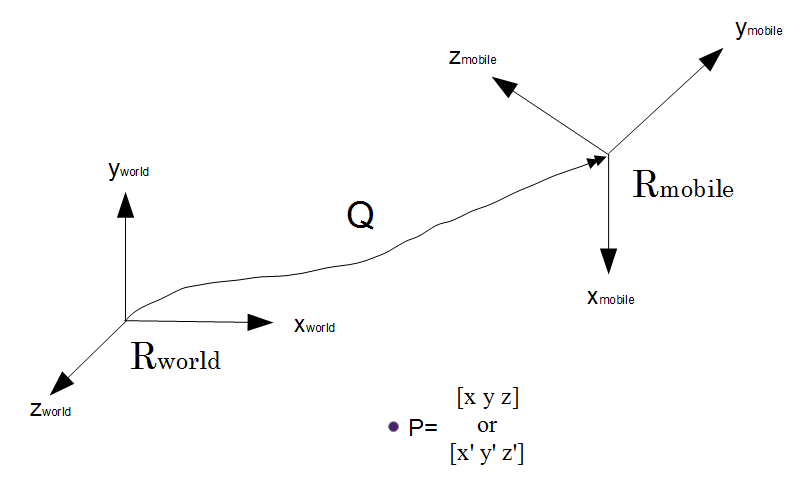
\includegraphics[width=12cm, keepaspectratio=true]{./Figures/coordinate_transformation/coordinate_transformation.png}
\caption{A point in world and mobile frame}
\label{fig:appx1-1}
\end{figure}

The two coordinate for point is related by
\begin{equation}
\begin{bmatrix}
x \\ y \\ z \\ 1 \\
\end{bmatrix}_{World}=Q\cdot\begin{bmatrix}
x' \\ y' \\ z' \\ 1  \\
\end{bmatrix}_{mobile}
\end{equation}

\noindent where Q is the transformation matrix composed by rotation
and translation evolve world frame to mobile frame. The calculation of
Q must follow the TRPY (translate-roll-pitch-yaw) convention, hence Q
is given by

\begin{equation}
Q=Q_T(x_T, y_T, z_T)Q_{Rz}(r_{z})Q_{Ry}(r_{y}) 
Q_{Rx}(r_{x})
\end{equation}

$Q_T(x_T, y_T, z_T)$, $Q_{R_x}$, $Q_{R_y}$, $Q_{R_z}$ is the
translation and rotation matrix for axis $X$, $Y$ and $Z$. They are
give in equation (\ref{eq:translate}) to (\ref{eq:rotz}). 

\begin{equation}
\label{eq:translate}
Q_T(x_T, y_T, z_T) = \begin{bmatrix}
1 & 0 & 0 & x_T \\
0 & 1 & 0 & y_T \\
0 & 0 & 1 & z_T \\
0 & 0 & 0 & 1 \end{bmatrix}
\end{equation}

\begin{equation}
\label{eq:rotx}
Q_{Rx}(r_{x})=\lbrack \begin{bmatrix}
1 & 0 & 0 & 0 & \\
0 & \cos (r_{x}) & -\sin (r_{x}) & 0 & \\
0 & \sin (r_{x}) & \cos (r_{x}) & 0 & \\
0 & 0 & 0 & 1 & \\
\end{bmatrix}
\end{equation}


\begin{equation}
\label{eq:roty}
Q_{Ry}(r_{y})= \begin{bmatrix}
\cos (r_{y}) & 0 & \sin (r_{y}) & 0 & \\
0 & 1 & 0 & 0 & \\
-sin(r_{y}) & 0 & \cos (r_{y}) & 0 & \\
0 & 0 & 0 & 1 & 
\end{bmatrix}
\end{equation}


\begin{equation}
\label{eq:rotz}
Q_{Rz}(r_{z})=\begin{bmatrix}
\cos (r_{z}) & -\sin (r_{z}) & 0 & 0 & \\
\sin (r_{z}) & \cos (r_{z}) & 0 & 0 & \\
0 & 0 & 1 & 0 & \\
0 & 0 & 0 & 1 & \\
\end{bmatrix}
\end{equation}

The forward transformation calculate point $P$'s coordinate in world
frame given its location in mobile frame. To calculate point $P$'s
coordinate in mobile frame give its location is known in world frame.
inverse transformation can be used. The inverse transformation matrix
formula is give in equation (\ref{eq:Qinv}) - (\ref{eq:rotz_inv})

\begin{equation}
\label{eq:Qinv}
Q^{-1}=Q_{Rx}^{-1} Q_{Ry}^{-1} Q_{Rz}^{-1} Q_T^{-1}
\end{equation}

\begin{equation}
\label{eq:translate_inv}
Q_{T}^{-1}=\begin{bmatrix}
1 & 0 & 0 & -x_T \\
0 & 1 & 0 & -y_T \\
0 & 0 & 1 & -z_T \\
0 & 0 & 0 & 1\end{bmatrix}
\end{equation}

\begin{equation}
\label{eq:rotx_inv}
Q_{Rx}^{-1}=Q_{Rx}^{T}
\end{equation}

\begin{equation}
\label{eq:roty_inv}
Q_{Ry}^{-1}=Q_{Ry}^{T}
\end{equation}

\begin{equation}
\label{eq:rotz_inv}
Q_{Rz}^{-1}=Q_{Rz}^{T}
\end{equation}




%%% Local Variables:
%%% mode: latex
%%% TeX-master: "thesis"
%%% End:
